\documentclass[]{article}
\usepackage{amsmath}
\usepackage{amsfonts}
\usepackage{graphicx}
\usepackage{booktabs}
\usepackage{fancyvrb}
\usepackage{array}
\usepackage{float}
\usepackage{xcolor}
\usepackage{xparse}
\usepackage{caption}
\usepackage{subcaption}
\usepackage{float}
\usepackage{multirow}
\usepackage{enumitem}
\usepackage{tikz}
\usepackage{ifthen}
\usepackage[T1]{fontenc}
\usepackage{hyperref}
\usepackage{rotating}

\def\UrlBreaks{\do\/\do-}

\newcommand{\cL}{{\cal L}}
\usetikzlibrary{matrix,arrows,positioning,shadows,automata,positioning}
\tikzset{
	feature/.style={draw, inner sep=1.0mm, font=\normalfont\sffamily, fill=white, drop shadow, align=center, auto},
	opt/.style={fill=white},
	man/.style={fill=black}
}

\newcommand{\connectfeaturesii}[3]{
	\draw (#2.south) -- (#3.north);
	\draw[#1] (#3.north) circle (.9mm);
}

\newcommand{\connectfeaturesiii}[4]{
	\ifthenelse{\equal{#1}{xor}}
	{
		\connectfeaturesii{opt}{#2}{#3};
		\connectfeaturesii{opt}{#2}{#4};
		\begin{scope}
			\path[clip] (#2.south) -- (#3.north) -- (#4.north);
			\draw (#2.south) circle (.5cm);
		\end{scope}
	}{
		\connectfeaturesii{man}{#2}{#3};
		\connectfeaturesii{man}{#2}{#4};
		\begin{scope}
			\path[clip] (#2.south) -- (#3.north) -- (#4.north);
			\fill[draw] (#2.south) circle (.5cm);
		\end{scope}
	}
}

\begin{document}

\begin{figure}[H]
	\centering
	\resizebox{0.8\textwidth}{!}{
		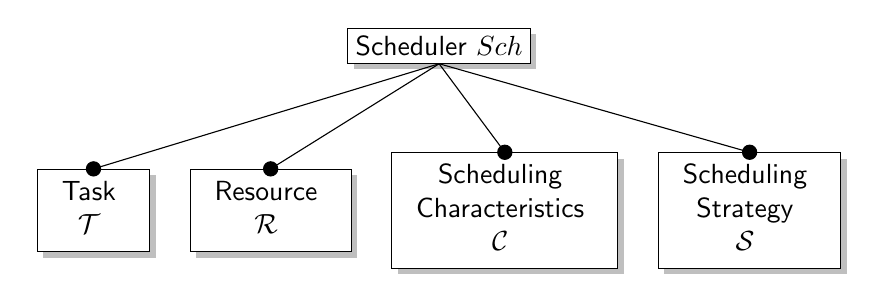
\begin{tikzpicture}[ampersand replacement=\&]
			\node[feature] (scheduler) {Scheduler $Sch$};
			
			\matrix (sub-scheduler)[matrix of nodes,
					  below=1cm of scheduler,
					  column sep=5mm, row sep=0mm, nodes=feature]{
				\begin{tabular}{c} Task \\ $\mathcal{T}$ \end{tabular} \& %sub-scheduler-1-1
				\begin{tabular}{c} Resource \\ $\mathcal{R}$ \end{tabular}  \& %sub-scheduler-1-2
				\begin{tabular}{c} Scheduling \\ Characteristics \\ $\mathcal{C}$ \end{tabular} \& %sub-scheduler-1-3
				\begin{tabular}{c} Scheduling \\ Strategy \\ $\mathcal{S}$ \end{tabular} \\ %sub-scheduler-1-4
			};
			
			\draw (scheduler.south) -- (sub-scheduler-1-1.north) ; \draw[man] (sub-scheduler-1-1.north) circle (.9mm);
			\draw (scheduler.south) -- (sub-scheduler-1-2.north) ;\draw[man] (sub-scheduler-1-2.north) circle (.9mm);
			\draw (scheduler.south) -- (sub-scheduler-1-3.north) ;\draw[man] (sub-scheduler-1-3.north) circle (.9mm);
			\draw (scheduler.south) -- (sub-scheduler-1-4.north) ;\draw[man] (sub-scheduler-1-4.north) circle (.9mm);
			
		\end{tikzpicture}
	}
	\caption{A configured \emph{Scheduler} feature model for OSP.}
\end{figure}
\begin{figure}[H]
	\centering
	\resizebox{1.2\textwidth}{!}{
		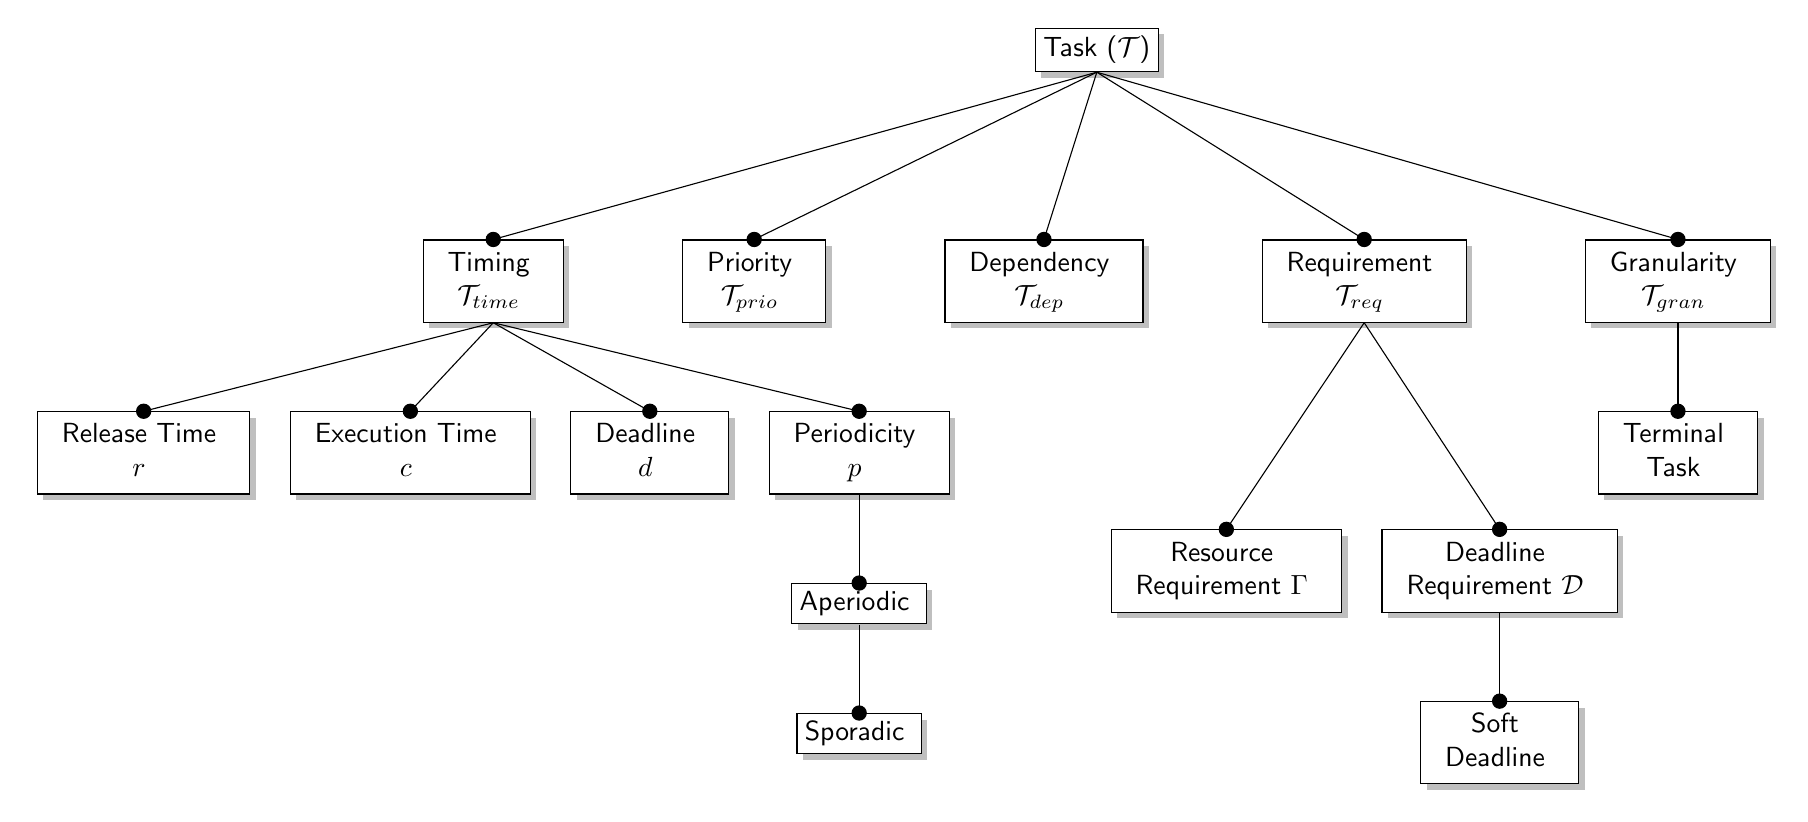
\begin{tikzpicture}[ampersand replacement=\&]
			\node[feature] (sub-scheduler) {Task ($\mathcal{T}$)};
			
			\matrix (task)[matrix of nodes,
					  below=2cm of sub-scheduler,
					  column sep=15mm, row sep=0mm, nodes=feature]{
				\begin{tabular}{c} Timing \\ $\mathcal{T}_{time}$ \end{tabular} \& %task-1-1
				\begin{tabular}{c} Priority \\ $\mathcal{T}_{prio}$ \end{tabular}  \& %task-1-2
%				\begin{tabular}{c} Dependency \\ $\mathcal{T}_{dep}$ \end{tabular}  \& %task-1-3
				\begin{tabular}{c} Dependency \\ $\mathcal{T}_{dep}$ \end{tabular}  \& %task-1-3
				\begin{tabular}{c} Requirement \\ $\mathcal{T}_{req}$ \end{tabular}  \& %task-1-4
				\begin{tabular}{c} Granularity \\ $\mathcal{T}_{gran}$ \end{tabular}  \\ %task-1-5
%				\begin{tabular}{c} Objective \\ $\mathcal{T}_{obj}$ \end{tabular} \\ %task-1-6
			};
			
			% Timing sub-feature diagram is drawn
			\matrix (timing)[matrix of nodes,
					  below=of task-1-1,
					  column sep=5mm, row sep=0mm, nodes=feature]{
				\begin{tabular}{c} Release Time \\ $r$ \end{tabular} \& %timing-1-1
				\begin{tabular}{c} Execution Time \\ $c$ \end{tabular} \& %timing-1-2
				\begin{tabular}{c} Deadline \\ $d$ \end{tabular} \& %timing-1-3
				\begin{tabular}{c} Periodicity \\ $p$ \end{tabular} \\ %timing-1-4
			};
			
			\matrix (periodicity)[matrix of nodes,
					  below=of timing-1-4,
					  column sep=5mm, row sep=0mm, nodes=feature]{
%				Periodic \& %periodicity-1-1
				Aperiodic \\ %periodicity-1-2
			};
			
			\matrix (aperiodic)[matrix of nodes,
		  			below=of periodicity-1-1,
		  			column sep=5mm, row sep=0mm, nodes=feature]{
				Sporadic \\ %periodicity-1-2
			};
			
			\connectfeaturesii{man}{sub-scheduler}{task-1-1};
			\connectfeaturesii{man}{sub-scheduler}{task-1-2};
			\connectfeaturesii{man}{sub-scheduler}{task-1-3};
			\connectfeaturesii{man}{sub-scheduler}{task-1-4};
			\connectfeaturesii{man}{sub-scheduler}{task-1-5};
			
			\connectfeaturesii{man}{task-1-1}{timing-1-1};
			\connectfeaturesii{man}{task-1-1}{timing-1-2};
			\connectfeaturesii{man}{task-1-1}{timing-1-3};
			\connectfeaturesii{man}{task-1-1}{timing-1-4};
			
			\connectfeaturesii{man}{timing-1-4}{periodicity-1-1};
			
			\connectfeaturesii{man}{periodicity-1-1}{aperiodic-1-1};
			
			% Preemtable sub-feature diagram is drawn
%			\matrix (preemptable)[matrix of nodes,
%					below=of task-1-3,
%					column sep=5mm, row sep=0mm, nodes=feature]{
%				Cooperative \\ %preemptable-1-1
%			};
			
%			\connectfeaturesii{man}{task-1-3}{preemptable-1-1};
			
			% Requirement sub-feature diagram is drawn
			\matrix (requirement)[matrix of nodes,
					below=2.5cm of task-1-4,
					column sep=5mm, row sep=0mm, nodes=feature]{
				\begin{tabular}{c} Resource \\ Requirement $\Gamma$ \end{tabular} \& %requirement-1-1
%				\begin{tabular}{c} Mutex \\ Requirement $\mathcal{B}$ \end{tabular} \& %requirement-1-2
				\begin{tabular}{c} Deadline \\ Requirement $\mathcal{D}$ \end{tabular} \\ %requirement-1-3
			};
			
			\matrix (deadline-requirement)[matrix of nodes,
								below=of requirement-1-2,
								column sep=5mm, row sep=0mm, nodes=feature]{
%				\begin{tabular}{c} Hard \\ Deadline \end{tabular} \& %deadline-requirement-1-1
%				\begin{tabular}{c} Firm \\ Deadline \end{tabular} \& %deadline-requirement-1-2
				\begin{tabular}{c} Soft \\ Deadline \end{tabular} \\ %deadline-requirement-1-3
			};
			
			\connectfeaturesii{man}{task-1-4}{requirement-1-1};
%			\connectfeaturesii{opt}{task-1-4}{requirement-1-2};
			\connectfeaturesii{man}{task-1-4}{requirement-1-2};
			
			\connectfeaturesii{man}{requirement-1-2}{deadline-requirement-1-1};
			
%			\connectfeaturesiii{xor}{requirement-1-3}{deadline-requirement-1-1}{deadline-requirement-1-3};
			
			% Granularity sub-feature diagram is drawn
			\matrix (granularity)[matrix of nodes,
					below=of task-1-5,
					column sep=5mm, row sep=0mm, nodes=feature]{
%				\begin{tabular}{c} Terminal \\ Task \end{tabular} \& %granularity-1-1
				\begin{tabular}{c} Terminal \\ Task \end{tabular} \\ %granularity-1-2
			};
			
			\connectfeaturesii{man}{task-1-5}{granularity-1-1};
			
			% Objective sub-feature diagram is drawn
%			\matrix (objective-task)[matrix of nodes,
%					below=of task-1-6,
%					column sep=5mm, row sep=0mm, nodes=feature]{
%				Maximize \& %objective-task-1-1
%				Minimize \& %objective-task-1-2
%				Criteria \\ %objective-task-1-3
%			};
%			
%			\connectfeaturesiii{xor}{task-1-6}{objective-task-1-1}{objective-task-1-2};
%			\connectfeaturesii{man}{task-1-6}{objective-task-1-3};
			
		\end{tikzpicture}
	}
	\caption{A configured \emph{Task} sub-feature model for FSP.}
\end{figure}
\begin{figure}[H]
	\centering
	\resizebox{1.\textwidth}{!}{
		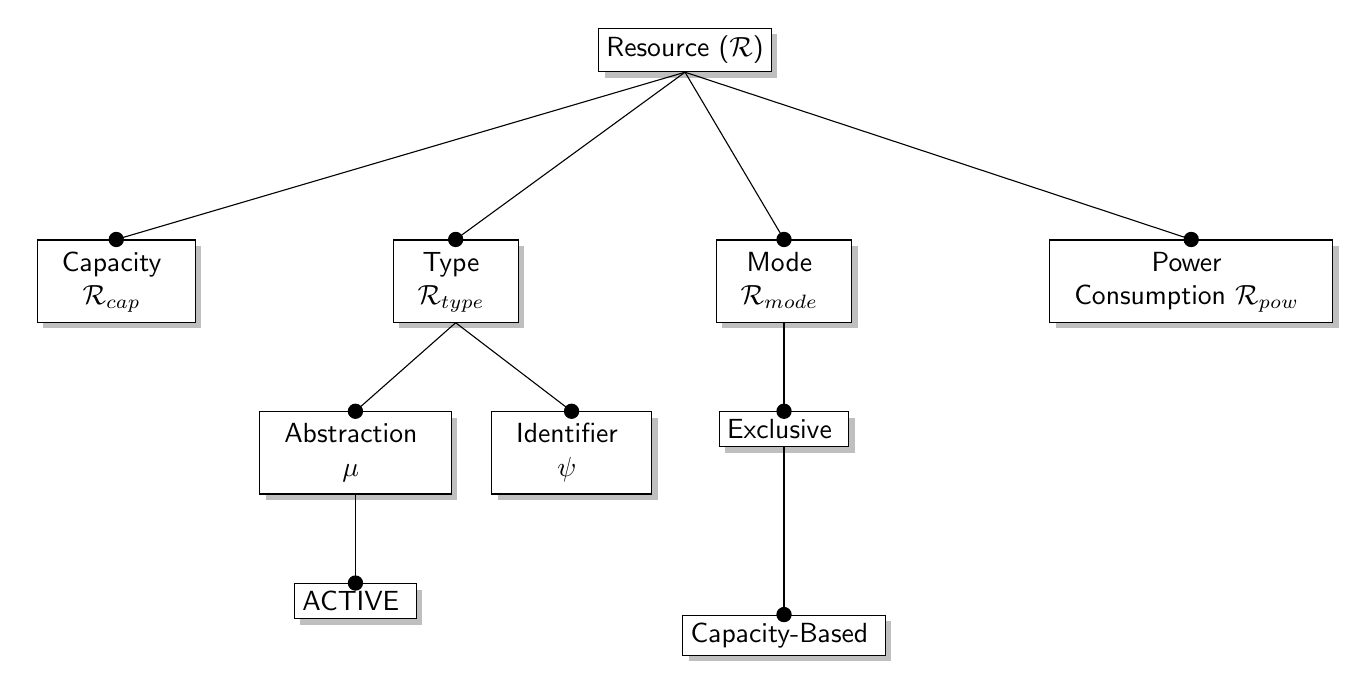
\begin{tikzpicture}[ampersand replacement=\&]
			\node[feature] (sub-scheduler) {Resource ($\mathcal{R}$)};
			
			\matrix (resource)[matrix of nodes,
					  below=2cm of sub-scheduler,
					  column sep=25mm, row sep=0mm, nodes=feature]{
				\begin{tabular}{c} Capacity \\ $\mathcal{R}_{cap}$ \end{tabular} \& %resource-1-1
				\begin{tabular}{c} Type \\ $\mathcal{R}_{type}$ \end{tabular}  \& %resource-1-2
				\begin{tabular}{c} Mode \\ $\mathcal{R}_{mode}$ \end{tabular}  \& %resource-1-3
				\begin{tabular}{c} Power \\ Consumption $\mathcal{R}_{pow}$ \end{tabular}  \\ %resource-1-4
%				\begin{tabular}{c} Objective \\ $\mathcal{R}_{obj}$ \end{tabular} \\ %task-1-5
			};
			
			% Resource type sub feature diagram is drawn.
			\matrix (type)[matrix of nodes,
					below=of resource-1-2,
					column sep=5mm, row sep=0mm, nodes=feature]{
				\begin{tabular}{c} Abstraction \\ $\mu$ \end{tabular}  \& %type-1-1
				\begin{tabular}{c} Identifier \\ $\psi$ \end{tabular} \\ %type-1-2
			};
			
			\matrix (abstraction)[matrix of nodes,
					below=of type-1-1,
					column sep=5mm, row sep=0mm, nodes=feature]{
				 ACTIVE \\ %abstraction-1-1
%				 PASSIVE \& %abstraction-1-2
%				 COMPOSITE \\ %abstraction-1-3
			};
			
			\draw (sub-scheduler.south) -- (resource-1-1.north);\draw[man] (resource-1-1.north) circle (.9mm);
			\draw (sub-scheduler.south) -- (resource-1-2.north);\draw[man] (resource-1-2.north) circle (.9mm);
			\draw (sub-scheduler.south) -- (resource-1-3.north);\draw[man] (resource-1-3.north) circle (.9mm);
			\draw (sub-scheduler.south) -- (resource-1-4.north);\draw[man] (resource-1-4.north) circle (.9mm);
%			\draw (sub-scheduler.south) -- (resource-1-5.north);\draw[opt] (resource-1-5.north) circle (.9mm);
			
			\draw (resource-1-2.south) -- (type-1-1.north);\draw[man] (type-1-1.north) circle (.9mm);
			\draw (resource-1-2.south) -- (type-1-2.north);\draw[man] (type-1-2.north) circle (.9mm);
			
			\draw (type-1-1.south) -- (abstraction-1-1.north);\draw[man] (abstraction-1-1.north) circle (.9mm);
%			\draw (type-1-1.south) -- (abstraction-1-2.north);\draw[opt] (abstraction-1-2.north) circle (.9mm);
%			\draw (type-1-1.south) -- (abstraction-1-3.north);\draw[opt] (abstraction-1-3.north) circle (.9mm);
%			\begin{scope}
%				\path[clip] (type-1-1.south) -- (abstraction-1-1.north) -- (abstraction-1-3.north);
%				\draw (type-1-1.south) circle (.5cm);
%			\end{scope}
			
			% Mode sub-feature diagram is drawn.
			\matrix (mode)[matrix of nodes,
					below=of resource-1-3,
					column sep=5mm, row sep=0mm, nodes=feature]{
%				Shared  \& %mode-1-1
				Exclusive \\ %mode-1-2
			};
			
			\draw (resource-1-3.south) -- (mode-1-1.north);\draw[man] (mode-1-1.north) circle (.9mm);
%			\draw (resource-1-3.south) -- (mode-1-2.north);\draw[opt] (mode-1-2.north) circle (.9mm);
%			\begin{scope}
%				\path[clip] (resource-1-3.south) -- (mode-1-1.north) -- (mode-1-2.north);
%				\draw (resource-1-3.south) circle (.5cm);
%			\end{scope}
			
			\matrix (exclusive)[matrix of nodes,
					below= 2cm of mode-1-1,
					column sep=1mm, row sep=0mm, nodes=feature]{
				Capacity-Based \\ %exclusive-1-1
%				Semantic-Based \\ %exclusive-1-2
			};
%			\connectfeaturesiii{or}{mode-1-2}{exclusive-1-1}{exclusive-1-2};
			\connectfeaturesii{man}{mode-1-1}{exclusive-1-1}
			
			% Power Consumption sub feature model is drawn.
%			\matrix (powcons)[matrix of nodes,
%					below=of resource-1-4,
%					column sep=5mm, row sep=0mm, nodes=feature]{
%				Scalable \\ %powcons-1-1
%			};
%			
%			\matrix (scalable)[matrix of nodes,
%					below=of powcons-1-1,
%					column sep=1mm, row sep=0mm, nodes=feature]{
%				Fixed-State  \& %scalable-1-1
%				Continuous-State \\ %scalable-1-2
%			};
			
%			\draw (resource-1-4.south) -- (powcons-1-1.north);\draw[opt] (powcons-1-1.north) circle (.9mm);
%			
%			\draw (powcons-1-1.south) -- (scalable-1-1.north);\draw[opt] (scalable-1-1.north) circle (.9mm);
%			\draw (powcons-1-1.south) -- (scalable-1-2.north);\draw[opt] (scalable-1-2.north) circle (.9mm);
%			\begin{scope}
%				\path[clip] (powcons-1-1.south) -- (scalable-1-1.north) -- (scalable-1-2.north);
%				\draw (powcons-1-1.south) circle (.5cm);
%			\end{scope}
			
			% Objective sub-feature diagram is drawn
%			\matrix (objective-resource)[matrix of nodes,
%					below=of resource-1-5,
%					column sep=5mm, row sep=0mm, nodes=feature]{
%				Maximize \& %objective-resource-1-1
%				Minimize \& %objective-resource-1-2
%				Criteria \\ %objective-resource-1-3
%			};
%			
%			\connectfeaturesiii{xor}{resource-1-5}{objective-resource-1-1}{objective-resource-1-2};
%			\connectfeaturesii{man}{resource-1-5}{objective-resource-1-3};
			
		\end{tikzpicture}
	}
	\caption{A configured \emph{Resource} sub-feature model for RMS.}
\end{figure}
\begin{figure}[H]
	\hspace{-3.5cm}
	\resizebox{1.6\textwidth}{!}{
		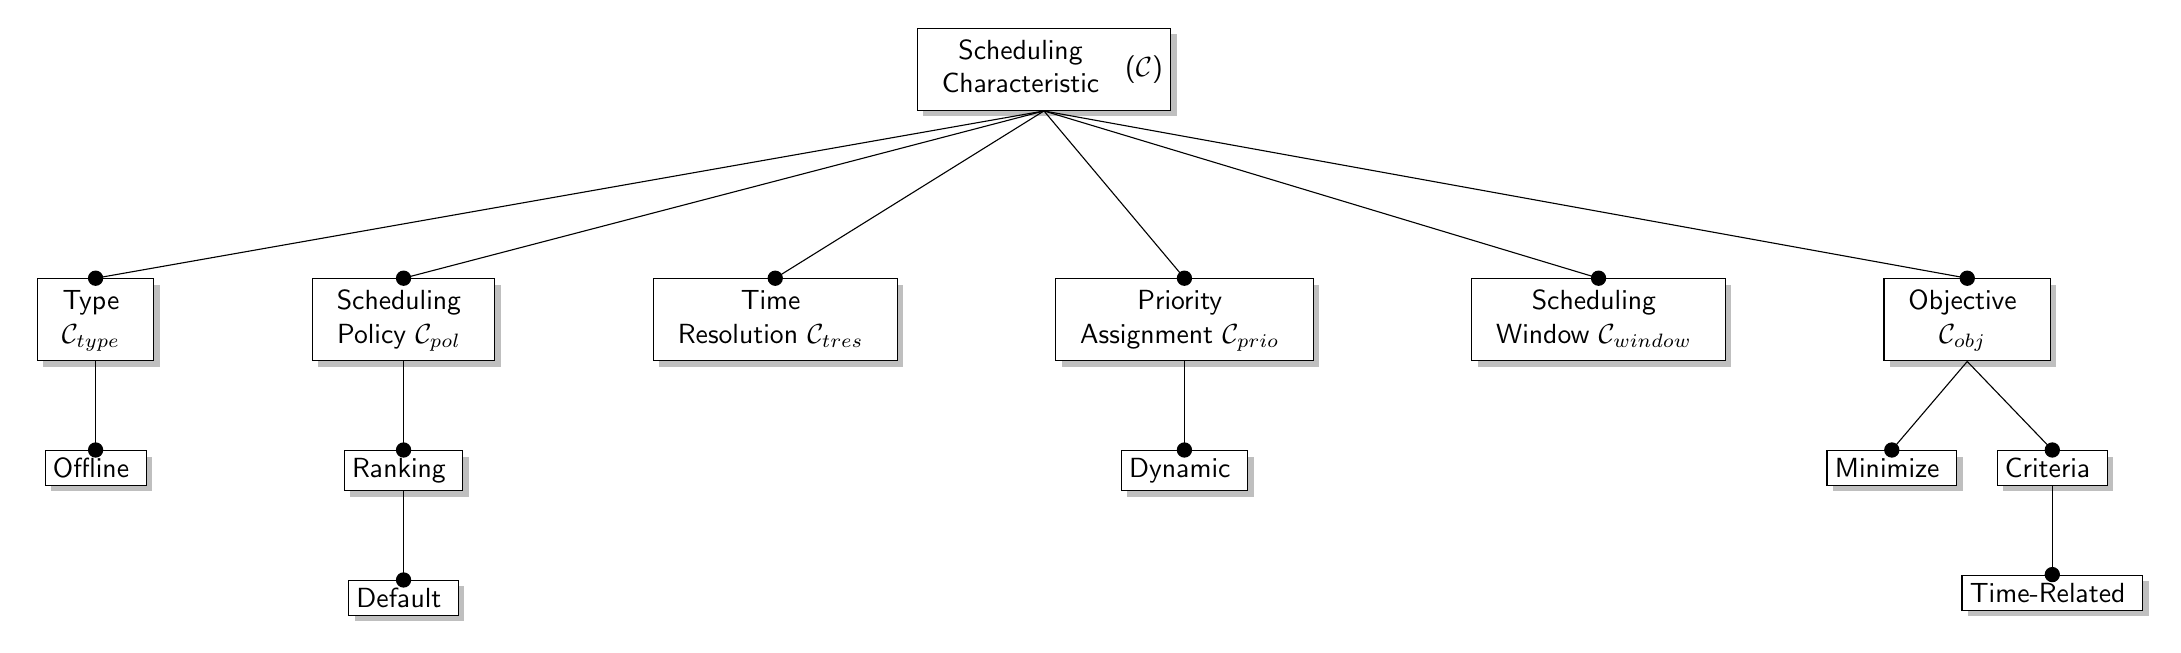
\begin{tikzpicture}[ampersand replacement=\&]
			\node[feature] (sub-sched-char) {\begin{tabular}{c} Scheduling \\ Characteristic \end{tabular} ($\mathcal{C}$)};
			
			\matrix (sched)[matrix of nodes,
					  below=2cm of sub-sched-char,
					  column sep=20mm, row sep=0mm, nodes=feature]{
				\begin{tabular}{c} Type \\ $\mathcal{C}_{type}$ \end{tabular} \& %sched-1-1
%				\begin{tabular}{c} Preemptive \\ $\mathcal{C}_{prmp}$ \end{tabular}  \& %sched-1-2
%				\begin{tabular}{c} Migration \\ $\mathcal{C}_{mig}$ \end{tabular}  \& %sched-1-3
				\begin{tabular}{c} Scheduling \\ Policy $\mathcal{C}_{pol}$ \end{tabular}  \& %sched-1-2
				\begin{tabular}{c} Time \\ Resolution $\mathcal{C}_{tres}$ \end{tabular}  \& %sched-1-3
				\begin{tabular}{c} Priority \\ Assignment $\mathcal{C}_{prio}$ \end{tabular} \& %sched-1-4
				\begin{tabular}{c} Scheduling \\ Window $\mathcal{C}_{window}$ \end{tabular} \& %sched-1-5
				\begin{tabular}{c} Objective \\ $\mathcal{C}_{obj}$ \end{tabular} \\ %sched-1-6
			};
			
			\connectfeaturesii{man}{sub-sched-char}{sched-1-1};
			\connectfeaturesii{man}{sub-sched-char}{sched-1-2};
			\connectfeaturesii{man}{sub-sched-char}{sched-1-3};
			\connectfeaturesii{man}{sub-sched-char}{sched-1-4};
			\connectfeaturesii{man}{sub-sched-char}{sched-1-5};
			\connectfeaturesii{man}{sub-sched-char}{sched-1-6};
			
			\matrix (type)[matrix of nodes,
					 below=of sched-1-1,
					 column sep=5mm, row sep=0mm, nodes=feature]{
%				Offline \& %type-1-1
				Offline \\ %type-1-2
			};
			
			\connectfeaturesii{man}{sched-1-1}{type-1-1};
			
%			\matrix (migration)[matrix of nodes,
%				 below=of sched-1-3,
%				 column sep=5mm, row sep=0mm, nodes=feature]{
%%				Task-level \& %migration-1-1
%				Job-level \\ %migration-1-2
%			};
%			\connectfeaturesii{man}{sched-1-3}{migration-1-1};
			
			\matrix (policy)[matrix of nodes,
					below=of sched-1-2,
					column sep=5mm, row sep=0mm, nodes=feature]{
%				Grouping \& %policy-1-1
				Ranking \\ %policy-1-2
			};
			\connectfeaturesii{man}{sched-1-2}{policy-1-1};
%			\connectfeaturesii{man}{sched-1-2}{policy-1-2};
			\matrix (ranking)[matrix of nodes,
					below=of policy-1-1,
					column sep=5mm, row sep=0mm, nodes=feature]{
				Default \\ %ranking-1-1
%				User-defined \\ %ranking-1-2
			};
			\connectfeaturesii{man}{policy-1-1}{ranking-1-1};
			
			\matrix (priority)[matrix of nodes,
					below=of sched-1-4,
					column sep=5mm, row sep=0mm, nodes=feature]{
				Dynamic \\ %priority-1-1
%				Dynamic \\ %priority-1-2
			};
			\connectfeaturesii{man}{sched-1-4}{priority-1-1};
			
			\matrix (sched-objective)[matrix of nodes,
					below=of sched-1-6,
					column sep=5mm, row sep=0mm, nodes=feature]{
%				Maximize \& %sched-objective-1-1
				Minimize \& %sched-objective-1-2
				Criteria \\ %sched-objective-1-3
			};
			\connectfeaturesii{man}{sched-1-6}{sched-objective-1-1}
			\connectfeaturesii{man}{sched-1-6}{sched-objective-1-2}
			
			\matrix (sched-criteria)[matrix of nodes,
			below=of sched-objective-1-2,
			column sep=5mm, row sep=0mm, nodes=feature]{
				Time-Related \\ %sched-criteria-1-1
%				Resource-Related \& %sched-criteria-1-2
%				Abstract \\ %sched-criteria-1-3
			};
			\connectfeaturesii{man}{sched-objective-1-2}{sched-criteria-1-1};
%			\connectfeaturesiii{or}{sched-objective-1-3}{sched-criteria-1-1}{sched-criteria-1-3};
		
		\end{tikzpicture}
	}
	\caption{A configured \emph{Scheduling Characteristics} sub-feature model for FSP.}
\end{figure}
\begin{figure}[H]
	\centering
	\resizebox{0.6\textwidth}{!}{
		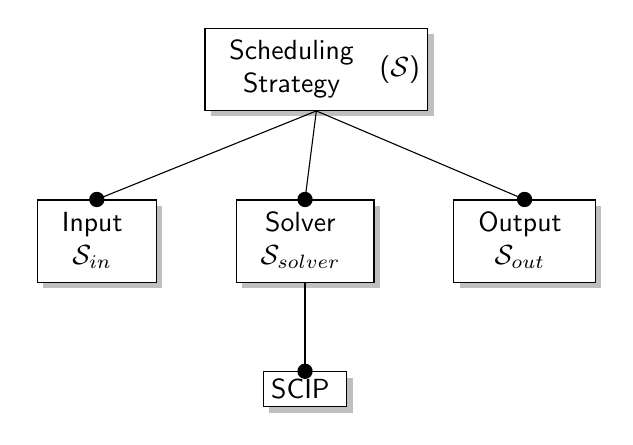
\begin{tikzpicture}[ampersand replacement=\&]
			\node[feature] (sub-sched-strategy) {\begin{tabular}{c} Scheduling \\ Strategy \end{tabular} ($\mathcal{S}$)};
			
			\matrix (sched)[matrix of nodes,
					  below=1cm of sub-sched-strategy,
					  column sep=10mm, row sep=0mm, nodes=feature]{
				\begin{tabular}{c} Input \\ $\mathcal{S}_{in}$ \end{tabular}  \& %sched-1-1
				\begin{tabular}{c} Solver \\ $\mathcal{S}_{solver}$ \end{tabular} \& %sched-1-2
				\begin{tabular}{c} Output \\ $\mathcal{S}_{out}$ \end{tabular}  \\ %sched-1-3
			};
			
			\connectfeaturesii{man}{sub-sched-strategy}{sched-1-1};
			\connectfeaturesii{man}{sub-sched-strategy}{sched-1-2};
			\connectfeaturesii{man}{sub-sched-strategy}{sched-1-3};
			
			\matrix (solver)[matrix of nodes,
					 below=of sched-1-2,
					 column sep=5mm, row sep=0mm, nodes=feature]{
				SCIP \\ %solver-1-1
%				MiniSat \& %solver-1-2
%				MipWrapper \& %solver-1-3
%				Mistral \& %solver-1-4
%				Mistral2 \& %solver-1-5
%				SatWrapper \& %solver-1-6
%				Toulbar2 \& %solver-1-7
%				Walksat \& %solver-1-8
%				Other \\ %solver-1-9
			};
			
%			\connectfeaturesiii{or}{sched-1-2}{solver-1-1}{solver-1-9};
			\connectfeaturesii{man}{sched-1-2}{solver-1-1};
%			\connectfeaturesii{man}{sched-1-2}{solver-1-3};
%			\connectfeaturesii{man}{sched-1-2}{solver-1-4};
%			\connectfeaturesii{man}{sched-1-2}{solver-1-5};
%			\connectfeaturesii{man}{sched-1-2}{solver-1-6};
%			\connectfeaturesii{man}{sched-1-2}{solver-1-7};
%			\connectfeaturesii{man}{sched-1-2}{solver-1-8};
		
%			\matrix (input)[matrix of nodes,
%					below=of sched-1-3,
%					column sep=5mm, row sep=0mm, nodes=feature]{
%				DSLB \& %input-1-1
%				DSB \\ %input-1-2
%			};
%			\connectfeaturesiii{or}{sched-1-3}{input-1-1}{input-1-2};
		
%			\matrix (output)[matrix of nodes,
%					below=of sched-1-4,
%					column sep=5mm, row sep=0mm, nodes=feature]{
%				DSLB \& %input-1-1
%				DSB \\ %input-1-2
%			};
%			\connectfeaturesiii{or}{sched-1-4}{output-1-1}{output-1-2};
		
		
		\end{tikzpicture}
	}
		\caption{A configured \emph{Scheduling Strategy} sub-feature model for JSP.}
\end{figure}


\end{document}
